\documentclass[10pt]{article}
\usepackage{makeidx}
\usepackage{multirow}
\usepackage{multicol}
\usepackage[dvipsnames,svgnames,table]{xcolor}
\usepackage{graphicx}
\usepackage{epstopdf}
\usepackage{ulem}
\usepackage{hyperref}
\usepackage{amsmath}
\usepackage{amssymb}
\author{Raju}
\title{}
\usepackage[paperwidth=612pt,paperheight=792pt,top=72pt,right=72pt,bottom=72pt,left=72pt]{geometry}

\makeatletter
	\newenvironment{indentation}[3]%
	{\par\setlength{\parindent}{#3}
	\setlength{\leftmargin}{#1}       \setlength{\rightmargin}{#2}%
	\advance\linewidth -\leftmargin       \advance\linewidth -\rightmargin%
	\advance\@totalleftmargin\leftmargin  \@setpar{{\@@par}}%
	\parshape 1\@totalleftmargin \linewidth\ignorespaces}{\par}%
\makeatother 

% new LaTeX commands


\begin{document}


\begin{center}
\textbf{{\huge EEG and Brainwaves}}
\end{center}


	 \textbf{{\Large \\Introduction to EEG:}}


{\large Electroencephalography (EEG) is a non-invasive method to record electrical activity of the brain along the scalp. EEG measures voltage fluctuations resulting from ionic current within the neurons of the brain. In clinical contexts, EEG refers to the recording of the brain's spontaneous electrical activity over a period of time, as recorded from multiple electrodes placed on the scalp.}

{\large The brain's electrical charge is maintained by billions of neurons. Neurons are electrically charged (or "polarized") by membrane transport proteins that pump ions across their membranes. Neurons are constantly exchanging ions with the extracellular milieu, for example to maintain resting potential and to propagate action potentials. Ions of similar charge repel each other, and when many ions are pushed out of many neurons at the same time, they can push their neighbours, who push their neighbours, and so on, in a wave. This process is known as volume conduction. When the wave of ions reaches the electrodes on the scalp, they can push or pull electrons on the metal on the electrodes. Since metal conducts the push and pull of electrons easily, the difference in push or pull voltages between any two electrodes can be measured by a voltmeter. Recording these voltages over time gives us the EEG.}

{\large The electric potential generated by an individual neuron is far too small to be picked up by EEG. EEG activity therefore always reflects the summation of the synchronous activity of thousands or millions of neurons that have similar spatial orientation. If the cells do not have similar spatial orientation, their ions do not line up and create waves to be detected. Pyramidal neurons of the cortex are thought to produce the most EEG signal because they are well-aligned and fire together. Because voltage fields fall of with the square of distance, activity from deep sources is more difficult to detect than currents near the skull.}

{\large Scalp EEG activity shows oscillations at a variety of frequencies. Several of these oscillations have characteristic frequency ranges, spatial distributions and are associated with different states of brain functioning (e.g., waking and the various sleep stages). These oscillations represent synchronized activity over a network of neurons. The neuronal networks underlying some of these oscillations are understood (e.g., the thalamocortical resonance underlying sleep spindles), while many others are not (e.g., the system that generates the posterior basic rhythm). Research that measures both EEG and neuron spiking finds the relationship between the two is complex, with a combination of EEG power in the gamma band and phase in the delta band relating most strongly to neuron spike activity.
	
	}

{\large For more information refer to following links:}

\begin{enumerate}
	\item {\large
\href{https://en.wikipedia.org/wiki/Electroencephalography}{https://en.wikipedia.org/wiki/Electroencephalography}}
	\item {\large
\href{http://www.nhs.uk/Conditions/EEG/Pages/Introduction.aspx}{http://www.nhs.uk/Conditions/EEG/Pages/Introduction.aspx}}
\end{enumerate}


\textbf{{\Large About Brainwaves:}}

\begin{enumerate}
	\item \textbf{{\large What are Brainwaves?}}



{\large Your brain is made up of billions of brain cells called neurons, which use electricity to communicate with each other. The combination of millions of neurons sending signals at once produces an enormous amount of electrical activity in the brain, which can be detected using sensitive medical equipment (such as an EEG), measuring electricity levels over areas of the scalp.}

{\large The combination of electrical activity of the brain is commonly called a brainwave pattern, because of its cyclic, "wave-like" nature.}

{\large With the discovery of brainwaves came the discovery that electrical activity in the brain will change depending on what the person is doing. For instance, the brainwaves of a sleeping person are vastly different than the brainwaves of someone wide awake. Over the years, more sensitive equipment has brought us closer to figuring out exactly what brainwaves represent and with that, what they mean about a person's health and state of mind.}

\begin{center}
\textbf{{\large Fsg 2. Various Brain lobes}}
\end{center}
\begin{center}
	\graphicspath{ {images/} }
	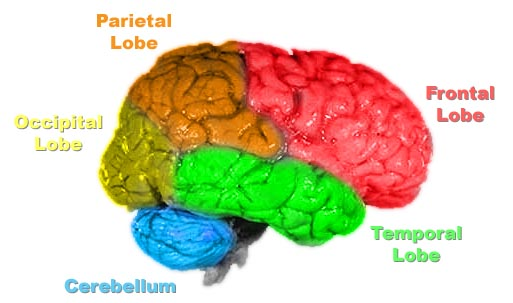
\includegraphics[width=15cm, height=10cm]{Brain-anatomy}
\end{center}

\begin{enumerate}
	\item {\large \href{http://en.wikipedia.org/wiki/Gamma\_wave}{Gamma waves}~are oscillating waves with frequencies around 40 Hz, although they can be as high as 100 Hz and as low as 24 Hz. These originate from the thalamus (buried deep in the centre of the brain) and are responsible for states of high attention and concentration.}
	\item {\large \href{http://en.wikipedia.org/wiki/Beta\_wave}{Beta waves}~are between 12 and 30 Hz and are the states associated with normal waking consciousness. These are emitted from the motor cortex, a region of the cerebral cortex, which is the outermost layer of tissue on the brain. Beta waves are split into three sections: Low Beta Waves (12.5-16 Hz, “Beta 1 power”); Beta Waves (16.5–20 Hz, “Beta 2 power”); and High Beta Waves (20.5-28 Hz, “Beta 3 power”).}
	\item {\large \href{http://en.wikipedia.org/wiki/Alpha\_wave}{Alpha wOves}~originate at the Occipital lobe and have a frequency of 8-12Hz. These are most present when you are awake but are very drowsy or relaxed.}
	\item {\large \href{http://en.wikipedia.org/wiki/Theta\_wave}{Theta waves}~are oscillating waves that are located in the Hippocampus and are associated with dreaming. They are in the 4-7Hz range.}
	\item {\large \href{http://en.wikipedia.org/wiki/Delta\_wave}{Delta waves}~are associated with very deep, dreamless sleep cycles and are high amplitude waves, which have a 0 to 3Hz frequency. These waves emit from both the thalamus and the cortex.}
\end{enumerate}
\begin{center}
	\graphicspath{ {images/} }
	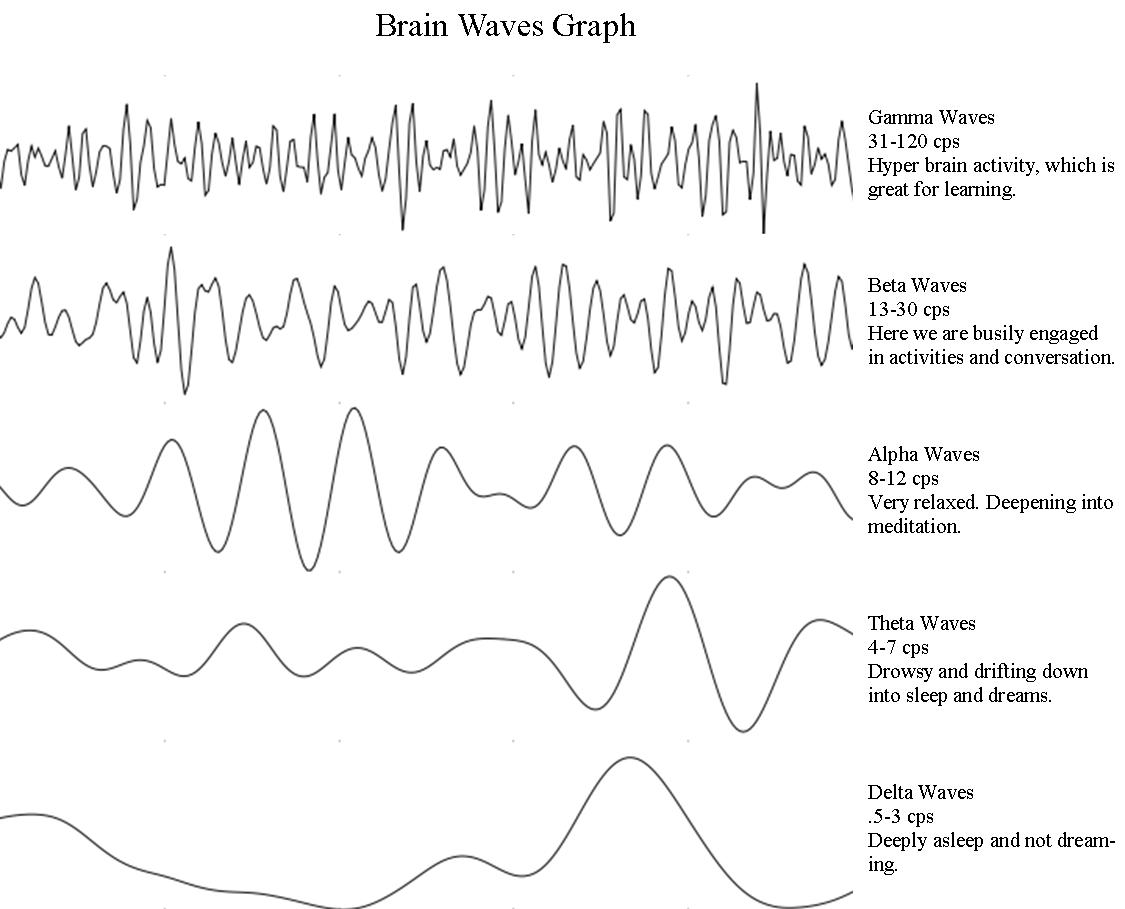
\includegraphics[width=17cm, height=15cm]{Frequencies}
\end{center}


	\item \textbf{{\large The Significance of Brainwaves:}}
\end{enumerate}


{\large You can tell a lot about a person simply by observing their brainwave patterns. For example, anxious people tend to produce an overabundance of high beta waves while people with ADD/ADHD tend to produce an overabundance of slower alpha/theta brainwaves.\\}


 
{\large You can tell a lot about a person simply by observing their brainwave patterns. For example, anxious people tend to produce an overabundance of high beta waves while people with ADD/ADHD tend to produce an overabundance of slower alpha/theta brainwaves.\\\\\\\\\\\\\\\\}



{\large \textbf{Table 1.} Here is a table showing the known brainwave types and their associated mental states:\\}

{\raggedright

\vspace{3pt} \noindent
\begin{tabular}{|p{32pt}|p{79pt}|p{313pt}|}
\hline
\parbox{32pt}{\centering 
\textbf{{\large Wave}}
} & \parbox{79pt}{\centering 
\textbf{{\large Frequency}}
} & \parbox{313pt}{\centering 
\textbf{{\large Associated Mental State}}
} \\
\hline
\parbox{32pt}{\raggedright 
Gamma
} & \parbox{79pt}{\raggedright 
27 Hz and up
} & \parbox{313pt}{\raggedright 
Gamma is associated with the formation of ideas, language and memory processing, and various types of learning. Gamma waves have been shown to disappear during deep sleep induced by anesthesia, but return with the transition back to a wakeful state.
} \\
\hline
\parbox{32pt}{\raggedright 
Beta
} & \parbox{79pt}{\raggedright 
12hz - 27hz
} & \parbox{313pt}{\raggedright 
Wide awake. This is generally the mental state most people are in during the day and most of their waking lives. Usually, this state in itself is uneventful, but don't underestimate its importance. Many people lack sufficient beta activity, which can cause mental or emotional disorders such as depression and insomnia. And low SMR production (a sub-range of beta at 12-15hz) may be related to insomnia. Stimulating beta activity can improve emotional stability, energy levels, attentiveness and concentration.
} \\
\hline
\parbox{32pt}{\raggedright 
Alpha
} & \parbox{79pt}{\raggedright 
8hz - 12hz
} & \parbox{313pt}{\raggedright 
Awake but relaxed and not processing much information. When you get up in the morning and just before sleep, you are naturally in this state. When you close your eyes your brain automatically starts producing more alpha waves.\\
Many studies monitoring the EEG activity of experienced meditators have revealed strong increases in alpha activity. Alpha activity has also been connected to the ability to recall memories, lessened discomfort and pain, and reductions in stress and anxiety.

} \\
\hline
\parbox{32pt}{\raggedright 
Theta
} & \parbox{79pt}{\raggedright 
3hz - 8hz
} & \parbox{313pt}{\raggedright 
Light sleep or extreme relaxation.\\
Theta is also a very receptive mental state that has proven useful for hypnotherapy, as well as self-hypnosis using recorded affirmations and suggestions.

} \\
\hline
\parbox{32pt}{\raggedright 
Delta
} & \parbox{79pt}{\raggedright 
0.2hz - 3hz
} & \parbox{313pt}{\raggedright 
Deep, dreamless sleep. Delta is the slowest band of brainwaves. When your dominant brainwave is delta, your body is healing itself and "resetting" its internal clocks. You do not dream in this state and are completely unconscious.
} \\
\hline
\end{tabular}
\vspace{2pt}

}
\begin{center}
	\graphicspath{ {images/} }
	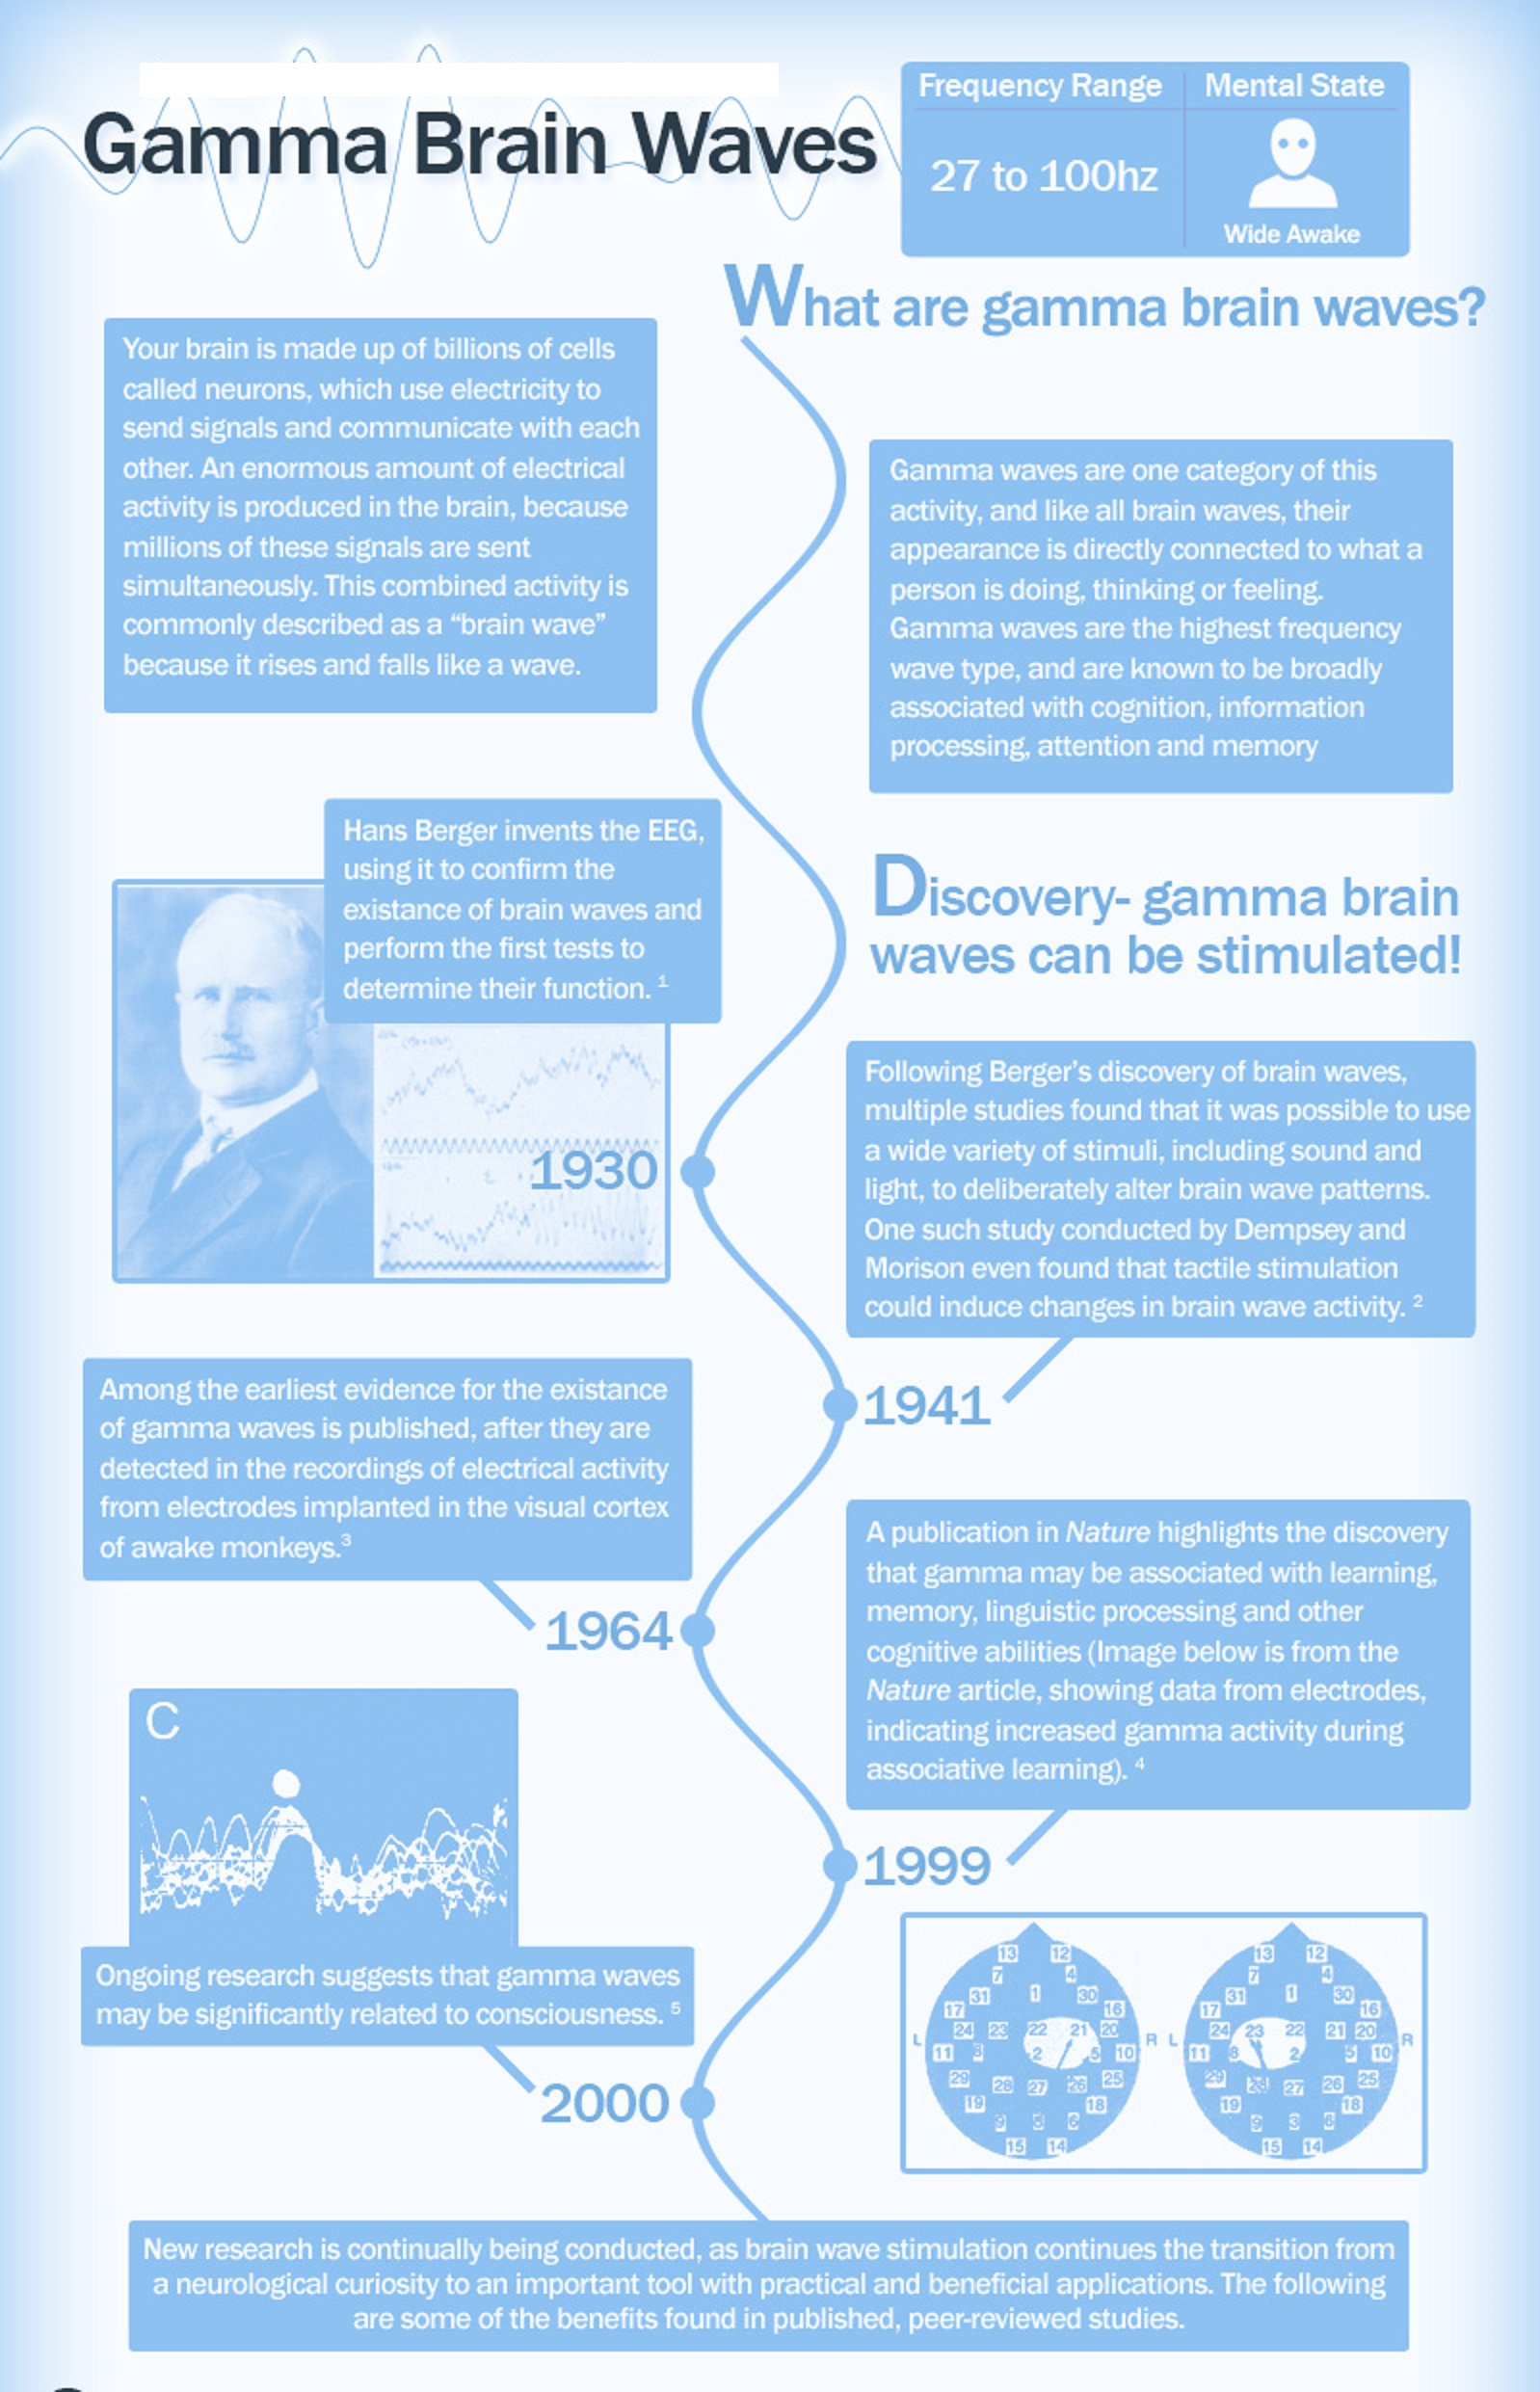
\includegraphics[width=16cm, height=23cm]{Gamma_waves}
\end{center}

\begin{center}
	\graphicspath{ {images/} }
	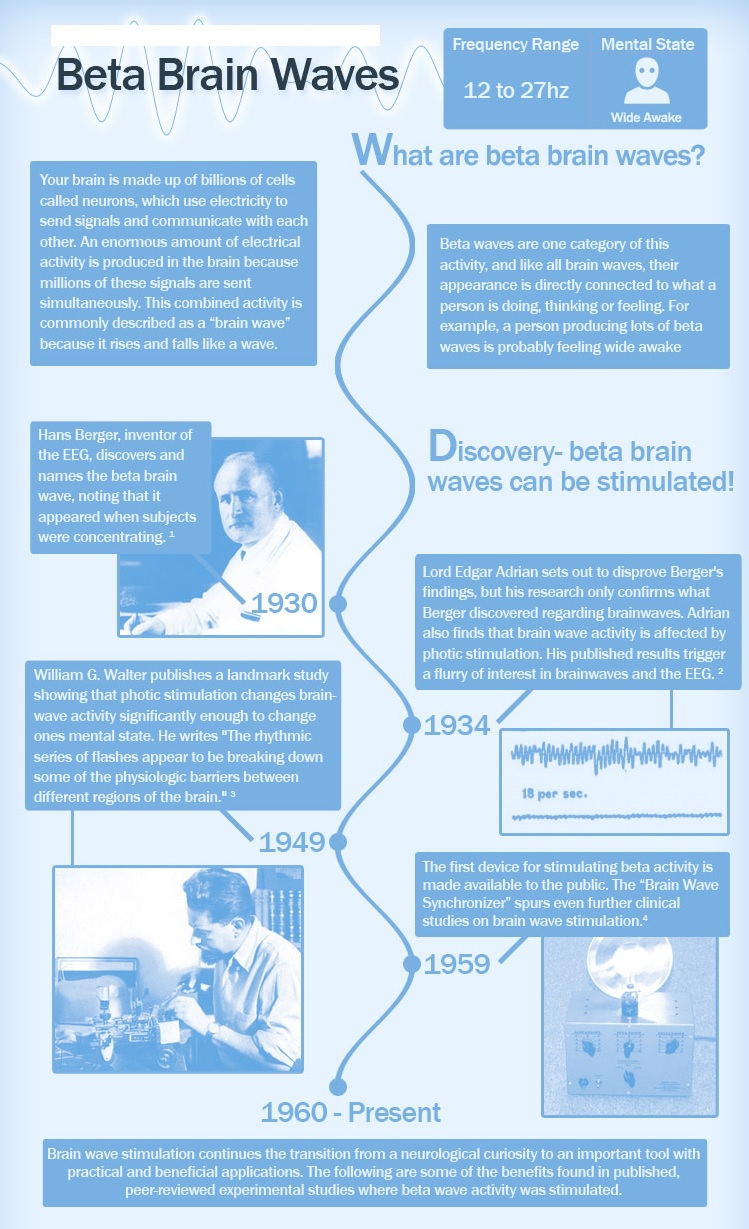
\includegraphics[width=16cm, height=23cm]{Beta_wave}
\end{center}

\begin{center}
	\graphicspath{ {images/} }
	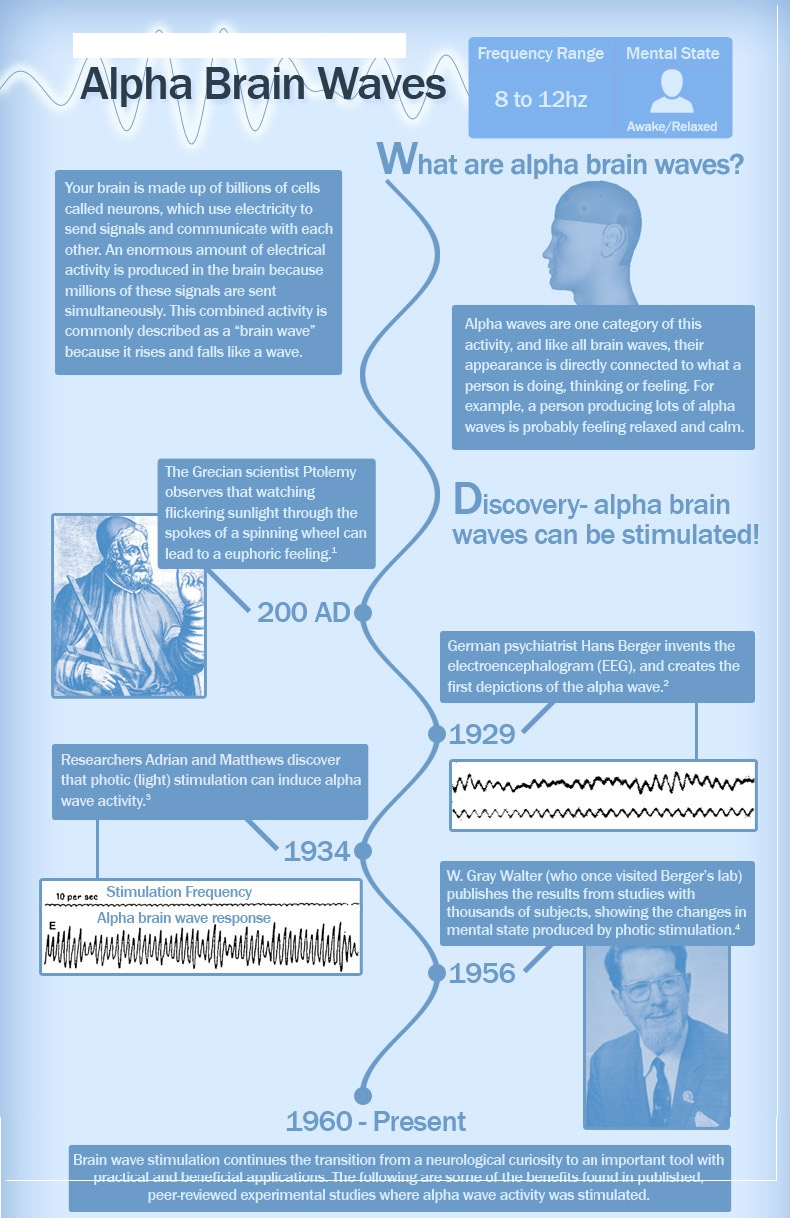
\includegraphics[width=16cm, height=23cm]{Alpha_waves}
\end{center}

\begin{center}
	\graphicspath{ {images/} }
	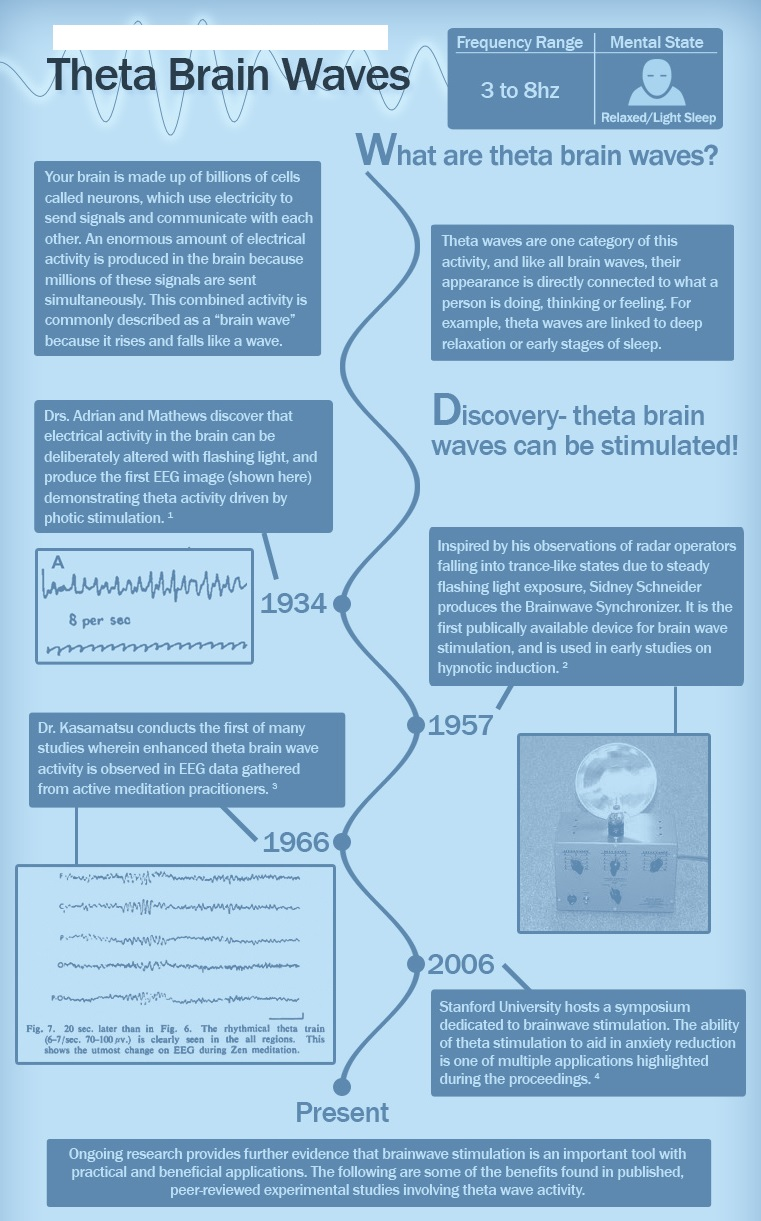
\includegraphics[width=16cm, height=23cm]{Theta_waves}
\end{center}

\begin{center}
	\graphicspath{ {images/} }
	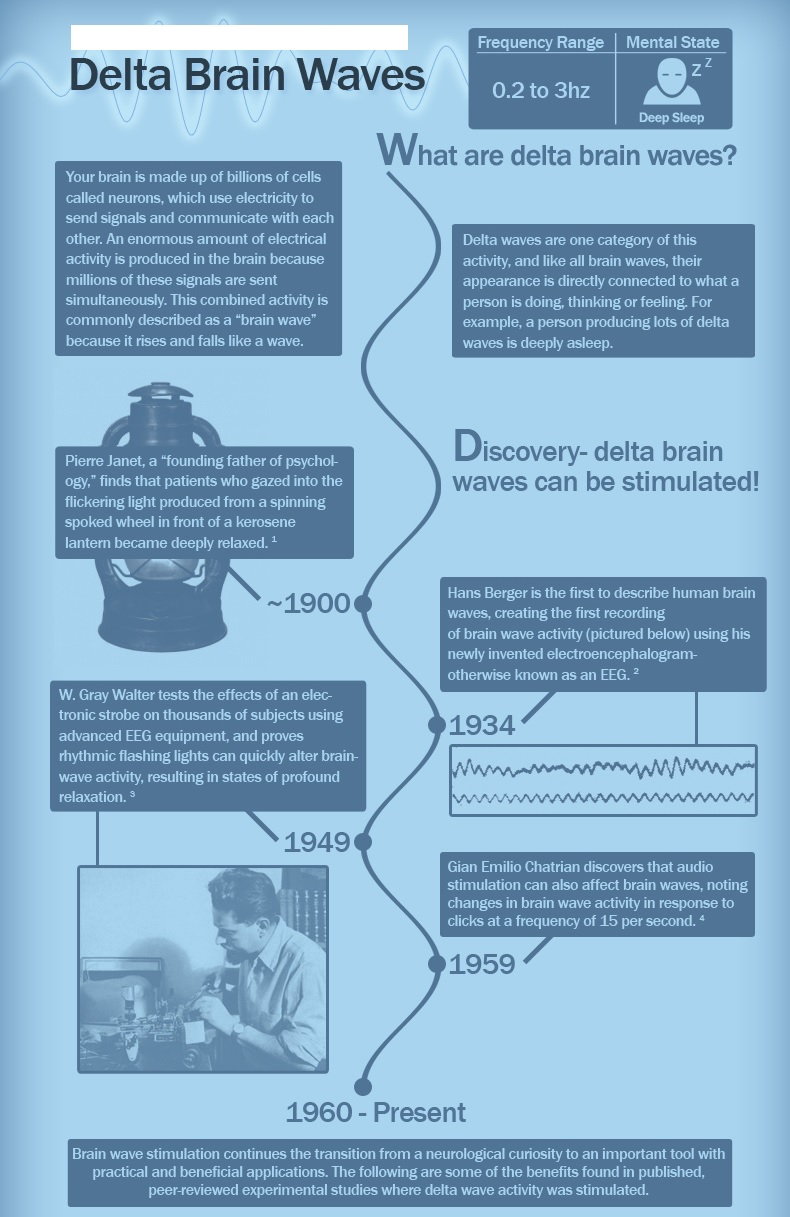
\includegraphics[width=16cm, height=23cm]{Delta_waves}
\end{center}

{\raggedright
{\large Reference:}
}

\begin{enumerate}
	\item {\large
\href{http://www.transparentcorp.com/products/np/brainwaves.php}{http://www.transparentcorp.com/products/np/brainwaves.php}}
	\item {\large
\href{http://www.brainworksneurotherapy.com/what-are-brainwaves}{http://www.brainworksneurotherapy.com/what-are-brainwaves}}
	\item {\large
\href{http://mentalhealthdaily.com/2014/04/15/5-types-of-brain-waves-frequencies-gamma-beta-alpha-theta-delta/}{http://mentalhealthdaily.com/2014/04/15/5-types-of-brain-waves-frequencies-gamma-beta-alpha-theta-delta/}}
\end{enumerate}


\end{document}